\chapter{Ejercicios Propuestos.}

\section{Ejercicios de Medicion}


\textbf{Ejercicio 1:} ¿Qué es la inversión según los economistas? Explique detalladamente.

Para los economistas la inversión puede ser englobada como aquel gasto en bienes de capital que sean activos \textbf{tangibles o intangibles} y puedan ser utilizados repetidas veces durante un año. También es importante que estén valorados a precio del comprador. Dentro la inversión podemos encontrar: inventarios y formación de capital fija, residencial fija y no residencial fija.

\textbf{Ejercicio 2:} Indique y justifique por que las siguientes afirmaciones son falsas o verdaderas:
\begin{enumerate}[(a)]
    \item Un buen modelo explica todo lo que pasa en una economía.
    
    Falso, no es necesario que para que una modelo sea "bueno" se necesite que explique todo lo que pasa en la economía. Para ello podemos asegurar que es necesario que reproduzca las características del fenómeno que se usó para estimarlo y capture elementos de los datos que no se usaron para estimarlo.
    \item Como los modelos hacen supuestos irreales, no sirven para estudiar la economía.
    
    Falso, los modelos de acuerdo a la rama epistémica de su estudio deben ser juzgado por la capacidad de predicciones no de la validez de sus supuestos. Muchos supuestos son relativamente irreales pues modelar la realidad sería imposible.
    
    \item Los modelos económicos no sirven para estudiar políticas económicas.
    
    Falso, 
    \item El mayor componente del PIB en Costa Rica es el gasto del gobierno.
    
    Falso, de acuerdo a los datos del Banco Central el mayor componente del PIB es el consumo general. Esto tiene mucho sentido económico pues el mayor porcentaje de activad económica en cual la mayoría de los agentes participa es en el consumo.
    
    \item Los modelos economicos ayudan a estudiar la respuesta de las variables exogenas.
    Falso
    
    \item  Costa Rica es una economía mas cerrada que Estados Unidos.
    Depende
    
    \item El PIB nominal no es una medida que funciona bastante bien para comparar cifras entre dos años diferentes. Explique detalladamente.
    Verdadero
    
    \item Si el PIB nominal y el índice de precios crecen a la misma tasa, los pobladores de una economía se encuentran aproximadamente igual de bien porque el PIB real no crece.
    Verdadero, 
    
    \item  El impuesto a los servicios transfronterizos (como Netflix) encarece los precios, por lo que causan inflacion.
    Falso,
    
    \item Una caída en la tasa de desempleo siempre augura buenas noticias para la economía. 
    Falso,
    
    \item Cuando el precio de un producto aumenta por mejoras en su calidad, este aumento
    debe aportar a la medicion de inflacion.
    Falso,
    
    \item Cuando un hogar sustituye servicios producidos en el hogar por servicios contratados en el mercado, el PIB no aumenta siempre y cuando el nivel de servicios disfrutados por el hogar se mantenga.
    Falso, 
\end{enumerate}

\textbf{Ejercicio 20: }Ingrese al sitio del Banco Central de Costa Rica (www.bccr.fi.cr) y descargue los datos de inflación de los últimos 10 a˜nos (es decir, 120 meses). Vamos a establecer algunos patrones estacionales de la inflación. Para ello, calcule la serie de la razón de la variación mensual sobre la variación interanual (es decir, variación mensual / variación interanual). Después, calcule el promedio mensual de cada uno de estas razones.

Considere la variaciones de la forma: 
\begin{align}
    \textup{Var. Mensual }&= \frac{P_{t}-P_{t-1}}{P_{t-1}}\\
    \textup{Var. Interanual }&= \frac{P_{t}-P_{t-12}}{P_{t-12}}\\
    \textup{Var. Mensual Anualizada }&= (P_{t}-P_{t-1})^{12}-1\\
    \textup{Var. Interanual Menlizada }&= (P_{t}-P_{t-1})^{\frac{1}{12}}-1
\end{align}

La razón de variaciones menciona como se comparta un mes en relación al comportamiento anual. 

\textbf{Respuestas:}
\begin{enumerate}[(a)]
    \item ¿Cúal es el máximo, mínimo y promedio de la variación porcentual mensual e interanual del IPC? Use las observaciones mensuales para esta pregunta.
    
    \begin{figure}[h]
        \centering
        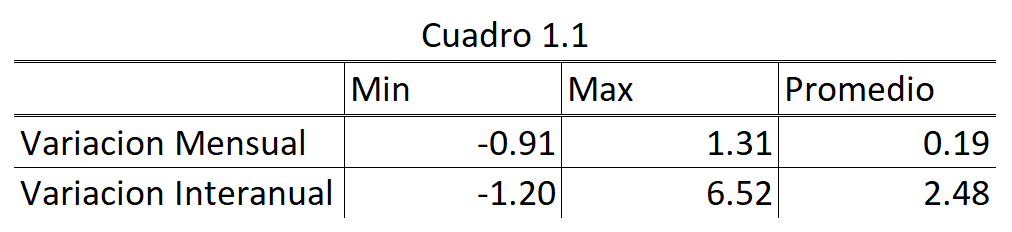
\includegraphics[scale=0.3]{Images/cuadro20.a.png}
        \caption{Respuesta 20.A}
        \label{fig:cuadro 20}
    \end{figure}
    
    \item  ¿Cuales son los dos meses con mayor relación mensual/interanual? Use los promedios mensuales de la muestra para esta pregunta.
    
    Los dos meses con mayor relación promedio son Julio y Diciembre.
    \item  ¿Cuales son los dos meses con menor relación mensual/interanual? Use los promedios mensuales de la muestra para esta pregunta.
    
    Los dos meses con menor relación promedio son Mayo y Enero.
    
    \item ¿Justifican estos datos hacer ajustes estacionales en los datos mensuales de inflación? Explique.
    
    Sí, la razón es que vemos que en estos meses es necesario hacer ajustes de estacionalidad dado a que durante estos meses, existen cambios culturales que impactan la forma de consumir de las personas. Incluyendo así diciembre como un periodo donde hay mayor gasto por compras de regalos y festividades.
    
    \item Tome las variaciones mensuales y anualícelas sin ajuste por estacionalidad (es decir,suponga que esa variación mensual se da por 12 meses seguidos). 
    
    \begin{figure}[h]
        \centering
        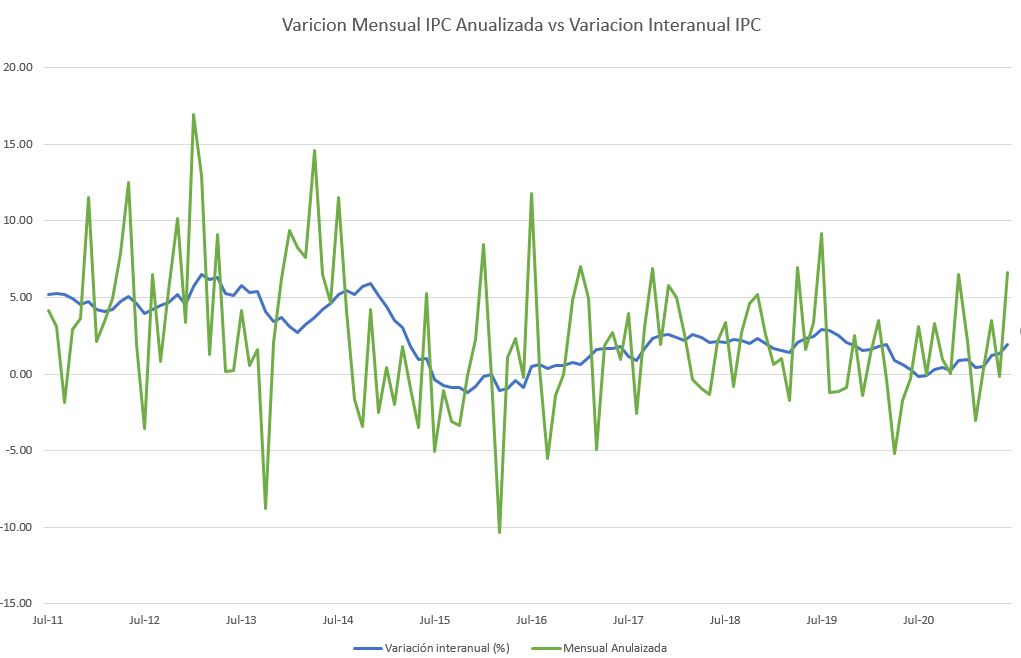
\includegraphics[scale = 0.5]{Images/VarMen_VarInt.png}
        \caption{Respuesta 20.E}
        \label{fig:cuadro 2}
    \end{figure}
    
$\blacksquare$
\end{enumerate}

\textbf{Ejercicio 21:} Ingrese al sitio web del Banco Central de Costa Rica (www.bccr.fi.cr) y descargue las siguientes tablas:
\begin{itemize}
    \item Índice de confianza sobre la actividad economica (ICAE, trimestral)
    \item Población total por condición de actividad y tasas (trimestral)
    \item Producto interno bruto y componentes del gasto (trimestral, desestacionalizado, volumen a precios del ano anterior encadenado)
    \item Índice de precios al consumidor (IPC, mensual)
    \item Credito del sistema bancario al sector privado no financiero por actividad economica (mensual)
\end{itemize}

\section{Ejercicios de Modelos IS-LM}
\textbf{Ejercicio 5:} Considere el siguiente modelo: 
\begin{equation}
  \begin{cases}
  C & =c_{0}+c_{1}(Y-T)\\
  I & = b_{0}+b_{1}Y -b_{2}i\\
  M^{d}/P & = d_{1}Y-d_{2}i
  \end{cases}  
\end{equation}

\begin{enumerate}[(a)]
    \item Halle el nivel de producción de equilibrio:

Asuma que $c_{1}+b_{1}<1$, entonces si $G$ es el componente del gasto de gobierno, y $Z=C+I+G$ es la demanda total de bienes y servicios en una economía cerrada. Se tiene entonces:
\begin{align}
    Z & = c_{0}+c_{1}(Y-T)+ b_{0}+b_{1}Y -b_{2}i+G\\
    & =  c_{0}+(c_{1}+b_{1})Y-c_{1}T+ b_{0} -b_{2}i+G
\end{align}
    
Si definimos el equilibrio del mercado de bienes y servicios es cuando la demanda total es igual a la producción
\begin{align}
    Z &= Y\\
    \implies & \nonumber \\
    Y &= c_{0}+(c_{1}+b_{1})Y-c_{1}T+ b_{0} -b_{2}i+G
\end{align}

Asi definimos que (5.9) es la relación \textbf{implicita} de la curva IS en esta economía. Si queremos buscar la curva LM podemos partir del supuesto que de que $M^{s}=M$ es la oferta monetaria y que es establecida de forma exógena por el Banco Central. El equilibrio en el mercado monetario es:
\begin{align}
    \frac{M^{d}}{P} &= M\\
    \implies & \nonumber \\
    M &= d_{1}Y-d_{2}i\\
    i & = \frac{d_{1}Y-M}{d_{2}}
\end{align}

En este caso (5.12) es la curva LM de nuestra economía. El nivel de producción para el cual se equilibrio nuestro mercado de bienes es:
\begin{align}
    Y &= c_{0}+(c_{1}+b_{1})Y-c_{1}T+ b_{0} -b_{2}\left(\frac{d_{1}Y-M}{d_{2}}\right)+G\\
    \left(1-c_{1}-b_{1}+\frac{b_{2}d_{1}}{d_{2}}\right)Y &
    = c_{0}-c_{1}T+ b_{0} +b_{2}\frac{M}{d_{2}}+G\\
    \left(\frac{d_{2}(1-c_{1}-b_{1})+b_{2}d_{1}}{d_{2}}\right)Y &
    = c_{0}-c_{1}T+ b_{0} +b_{2}\frac{M}{d_{2}}+G\\
    Y^{*} & = \frac{d_{2}(c_{0}-c_{1}T+ b_{0}+G) +b_{2}M}{d_{2}(1-c_{1}-b_{1})+b_{2}d_{1}}
\end{align}

\item Halle el tipo de interés de equilibrio

Para ello considere (5.12) y desarrolle de acuerdo a $Y^{*}$, entonces podemos plantearlo de la forma:
\begin{align}
        i^{*} & = \frac{d_{1}}{d_{2}}Y^{*}-\frac{M}{d_{2}}\\
         & = \frac{d_{1}}{d_{2}}\frac{d_{2}(c_{0}-c_{1}T+ b_{0}+G) +b_{2}M}{d_{2}(1-c_{1}-b_{1})+b_{2}d_{1}}-\frac{M}{d_{2}} \\
          & = \frac{d_{1}d_{2}(c_{0}-c_{1}T+ b_{0}+G) +d_{1}b_{2}M}{d_{2}\left[d_{2}(1-c_{1}-b_{1})+b_{2}d_{1}\right]}-\frac{\left[d_{2}(1-c_{1}-b_{1})+b_{2}d_{1}\right]M}{d_{2}\left[d_{2}(1-c_{1}-b_{1})+b_{2}d_{1}\right]}\\
         i^{*} & = \frac{d_{1}(c_{0}-c_{1}T+ b_{0}+G)-(1-c_{1}-b_{1})M}{\left[d_{2}(1-c_{1}-b_{1})+b_{2}d_{1}\right]}
\end{align}

\item Halle el nivel de inversión de equilibrio, para el manejo algebraico se complica más pues ahora debe considerar $i^{*}$ y $Y^{*}$ de la forma que:

\begin{align*}
    I^{*} &= b_{0}+b_{1}Y -b_{2}i \\
    & = b_{0}+b_{1}\left[\frac{d_{2}(c_{0}-c_{1}T+ b_{0}+G) +b_{2}M}{d_{2}(1-c_{1}-b_{1})+b_{2}d_{1}}\right]-b_{2}\left[\frac{d_{1}(c_{0}-c_{1}T+ b_{0}+G)-(1-c_{1}-b_{1})M}{\left[d_{2}(1-c_{1}-b_{1})+b_{2}d_{1}\right]}\right] \\
   I^{*} & = b_{0}+\frac{(c_{0}-c_{1}T+ b_{0}+G)(b_{1}d_{2}-b_{2}d_{1})+b_{2}M(1-c_{1})
    }{d_{2}(1-c_{1}-b_{1})+b_{2}d_{1}} 
\end{align*}
\item ¿En qué condiciones sobre los parámetros de modelo, aumenta la inversión cuando disminuye el gasto de gobierno?

Para ello podemos separar la función para poder aislar el componente del gasto, entonces para ellos establecemos:

\begin{equation}
    I^{*} = \frac{(1-c_{1})(b_{0}d_{2}+b_{2}M)+(b_{1}d_{2}-b_{2}d_{1})(c_{0}-c_{1}T)}{d_{2}(1-c_{1}-b_{1})+b_{2}d_{1}}+\frac{G(b_{1}d_{2}-b_{2}d_{1})}{d_{2}(1-c_{1}-b_{1})+b_{2}d_{1}}
\end{equation}

Suponga que se implementa politica fiscal por el laso del gasto, si todo permance igual, el cambio en la inversión esta dado por:

\begin{equation}
    \Delta I = \frac{\Delta G(b_{1}d_{2}-b_{2}d_{1})}{d_{2}(1-c_{1}-b_{1})+b_{2}d_{1}}
\end{equation}

Asuma entonces que si $\Delta G=-1$, entonces $\Delta I>0$ s.i.i

\begin{align}
    \frac{(b_{1}d_{2}-b_{2}d_{1})}{d_{2}(1-c_{1}-b_{1})+b_{2}d_{1}} & <0\\
    \nonumber \implies & \\
    (b_{1}d_{2}-b_{2}d_{1}) & <0 \\
    \frac{b_{1}}{b_{2}} & < \frac{d_{1}}{d_{2}}
\end{align}

\item Explique el inciso previo:

Considerando la política fiscal por vía del gasto afecta por dos razones, la primera por el aumento o disminución de las ventas de las empresas debido al aumento o disminución en la demanda total, y un efecto más indirecto que se da por el aumento en la da por el aumento de la tasa de interés ocasionada por la demanda de liquidez.

\begin{equation}
    I(Y(G), i(Y(G))) = b_{0}+b_{1}Y(G) -b_{2}i(Y(G)) \implies \frac{dI}{dG} = b_{1}\frac{dY}{dG}-b_{2}\frac{di}{dY}\frac{dY}{dG}
\end{equation}

Por ello entonces,

\begin{equation}
    b_{1}\frac{dY}{dG}-b_{2}\frac{di}{dY}\frac{dY}{dG} < 0 \implies \frac{b_{1}}{b_{2}} < \frac{di}{dY}
\end{equation}

Es decir, la condición nos dice que, para que esta política tenga un efecto positivo sobre la inversión, debe ser el caso de que el efecto por la disminución en las ventas del lado del mercado de bienes y servicios sea menor al efecto de la disminución en la tasa de interés por el lado del mercado monetario.

$\blacksquare$
\end{enumerate}